\section{Durchführung}
\label{sec:Durchführung}
\begin{figure}
    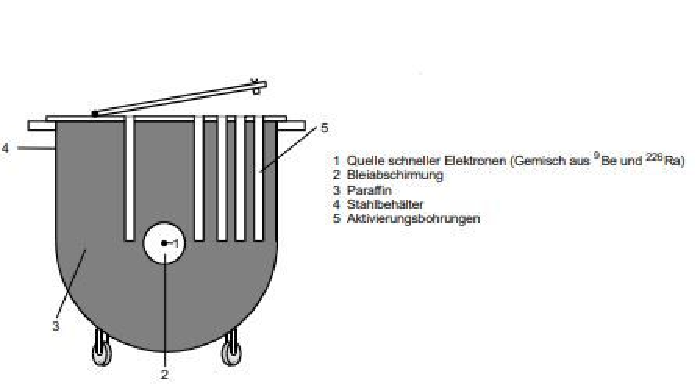
\includegraphics[width=\textwidth]{content/AufbauFoto.pdf}
    \caption{Versuchsaufbau vor Ort.\cite{anleitung}}
    \label{fig:AufbauFoto}
\end{figure}
Der Aufbau des Versuchs ist in Abbildung \ref{fig:AufbauFoto} mit den Messapparaturen zu sehen.
Zunächst wird der Nulleffekt mehrfach in Abständen von $\SI{300}{\second}$ gemessen.
\subsection{Vanadium}\label{subsec:vanadium}
Die Vanadium Probe wird aktiviert, aus der Neutronenquelle wieder entnommen und auf das Geiger-Müller-Zählrohr gesteckt.
Die Messung startet mit einem Messintervall von $\SI{30}{\second}$.
\subsection{Rhodium}
Ähnlich wie in Abschnitt \ref{subsec:vanadium} wird die Probe aktiviert, aus der Neutronenquelle entnommen und auf das Zählrohr gesteckt.
Diese Messung wird in einem Messintervall von $\SI{15}{\second}$ durchgeführt.